\documentclass[a4 paper]{article}
\usepackage[inner=2.0cm,outer=2.0cm,top=2.5cm,bottom=2.5cm]{geometry}
\usepackage{setspace}
\usepackage[rgb]{xcolor}
\usepackage{verbatim}
\usepackage{subcaption}
\usepackage{amsgen,amsmath,amstext,amsbsy,amsopn,tikz,amssymb}
\usepackage{fancyhdr}
\usepackage[colorlinks=true, urlcolor=blue,  linkcolor=blue, citecolor=blue]{hyperref}
\usepackage[colorinlistoftodos]{todonotes}
\usepackage{rotating}
\usepackage{booktabs}
\newcommand{\ra}[1]{\renewcommand{\arraystretch}{#1}}

\newtheorem{thm}{Theorem}[section]
\newtheorem{prop}[thm]{Proposition}
\newtheorem{lem}[thm]{Lemma}
\newtheorem{cor}[thm]{Corollary}
\newtheorem{defn}[thm]{Definition}
\newtheorem{rem}[thm]{Remark}
\numberwithin{equation}{section}

\newcommand{\homework}[6]{
   \pagestyle{myheadings}
   \thispagestyle{plain}
   \newpage
   \setcounter{page}{1}
   \noindent
   \begin{center}
   \framebox{
      \vbox{\vspace{2mm}
    \hbox to 6.28in { {\bf CSE 211:~Discrete Mathematics \hfill {\small (#2)}} }
       \vspace{6mm}
       \hbox to 6.28in { {\Large \hfill #1  \hfill} }
       \vspace{6mm}
       \hbox to 6.28in { {\it Instructor: {\rm #3} \hfill  {\rm #5} \hfill  {\rm #6}} \hfill}
       \hbox to 6.28in { {\it Assistant: #4  \hfill #6}}
      \vspace{2mm}}
   }
   \end{center}
   \markboth{#5 -- #1}{#5 -- #1}
   \vspace*{4mm}
}

\newcommand{\problem}[2]{~\\\fbox{\textbf{Problem #1}}\hfill (#2 points)\newline\newline}
\newcommand{\subproblem}[1]{~\newline\textbf{(#1)}}
\newcommand{\D}{\mathcal{D}}
\newcommand{\Hy}{\mathcal{H}}
\newcommand{\VS}{\textrm{VS}}
\newcommand{\solution}{~\newline\textbf{\textit{(Solution)}} }

\newcommand{\bbF}{\mathbb{F}}
\newcommand{\bbX}{\mathbb{X}}
\newcommand{\bI}{\mathbf{I}}
\newcommand{\bX}{\mathbf{X}}
\newcommand{\bY}{\mathbf{Y}}
\newcommand{\bepsilon}{\boldsymbol{\epsilon}}
\newcommand{\balpha}{\boldsymbol{\alpha}}
\newcommand{\bbeta}{\boldsymbol{\beta}}
\newcommand{\0}{\mathbf{0}}


\begin{document}
\homework{Homework \#3}{Due: 04/01/21}{Dr. Zafeirakis Zafeirakopoulos}{Gizem S\"ung\"u}{}{}
\textbf{Course Policy}: Read all the instructions below carefully before you start working on the assignment, and before you make a submission.
\begin{itemize}
\item It is not a group homework. Do not share your answers to anyone in any circumstance. Any cheating means at least -100 for both sides. 
\item Do not take any information from Internet.
\item No late homework will be accepted. 
\item For any questions about the homework, send an email to gizemsungu@gtu.edu.tr
\item The homeworks (both latex and pdf files in a zip file) will be
submitted into the course page of Moodle.
\item The latex, pdf and zip files of the homeworks should be saved as
"Name\_Surname\_StudentId".$\{$tex, pdf, zip$\}$.
\item If the answers of the homeworks have only calculations without any formula or any explanation -when needed- will get zero.
\item Writing the homeworks on Latex is strongly suggested. However, hand-written paper is still accepted $\textbf{IFF}$ hand writing of the student is clear and understandable to read, and the paper is well-organized. Otherwise, the assistant cannot grade the student's homework.
\end{itemize}

\problem{1: Representing Graphs}{10}
Represent the graph in Figure \ref{fig:graph1} with an adjacency matrix. Explain your representation clearly.
\begin{figure*}[htb]
	\centering
	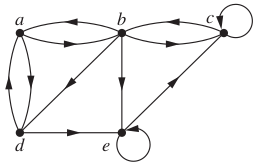
\includegraphics[scale=0.5]{graph1.png}
	\caption{The graph for Problem 1}
	\label{fig:graph1}
\end{figure*}
\solution
Since there are 5 nodes in the given graph, our matrix will be 5x5.We examine each edge individually. If there is a connection between the two edges, I make the value 1 in the matrix whichever direction it is. For example, there is a path between a and b, so I write 1 at the intersection of a and b in the matrix. Since there is no path between a and a, I make it 0 too.
\newline 
\begin{center}\hspace{5mm}a \hspace{2mm}b\hspace{2mm}    c\hspace{2mm}    d\hspace{2mm}    e 
\end{center}
\begin{equation*}
A =
\begin{pmatrix}
0 & 1 & 0 & 1 & 0 \\
1 & 0 & 1 & 1 & 1 \\
0 & 1 & 1 & 0 & 0 \\
1 & 0 & 0 & 0 & 1 \\
0 & 0 & 1 & 0 & 1 
\end{pmatrix}
\end{equation*}
\newpage
\problem{2: Hamilton Circuits}{10+10+10=30}
Determine whether there is a Hamilton circuit for each given graph (See Figure \ref{fig:G1a}, Figure \ref{fig:G1b}, Figure \ref{fig:G1c} ). If the graph has a Hamilton circuit, show the path with its vertices which gives a Hamilton circuit. If it does not, explain why no Hamilton circuit exists. \newline
\begin{figure*}[h]
	\centering
	\begin{subfigure}[h]{0.5\textwidth}
		\centering
		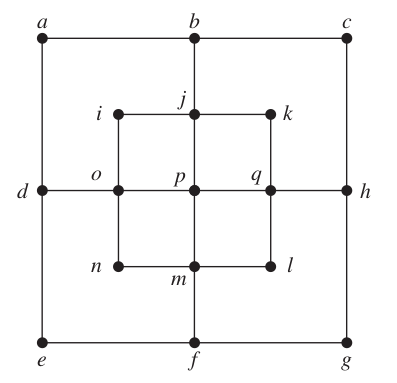
\includegraphics[height=1.5in]{circuit-a.png}
		\caption{The graph $G_1$}
		\label{fig:G1a}
	\end{subfigure}%
	\begin{subfigure}[h]{0.5\textwidth}
		\centering
		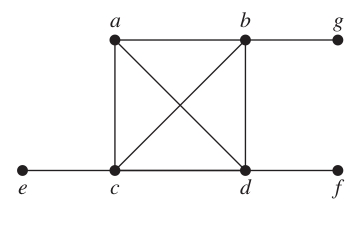
\includegraphics[height=1.5in]{circuit-b.png}
		\caption{The graph $G_2$}
		\label{fig:G1b}
	\end{subfigure}
	\begin{subfigure}[h]{0.5\textwidth}
		\centering
		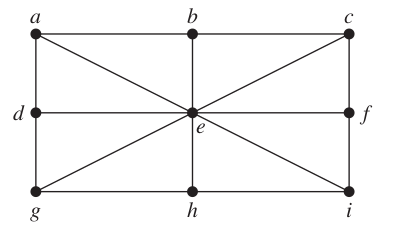
\includegraphics[height=1.2in]{circuit-c.png}
		\caption{The graph $G_3$}
		\label{fig:G1c}
	\end{subfigure}
	\caption{The graphs to find Hamilton circuits for Problem 1}
\end{figure*}

\subproblem{a} \solution
No Hamilton circuit exists.
\newline Reason : It must include both edges incident on vertices of degree two. It implies that must include 16 edges incident
\subproblem{b} \solution
No Hamilton circuit exists.
\newline Reason : Since there are three vertices of degree 1 in given graph so Hamilton circuit can't exist.
\subproblem{c} \solution
Yes. Hamilton circuit exists. The circuit is :

\newpage
\problem{3: Applications on Graphs}{20}
Schedule the final exams for Math 101, Math 243, CSE 333, CSE 346, CSE 101, CSE 102, CSE 273, and CSE 211, using the fewest number of different time slots, if there are no students who are taking:
\begin{itemize}
	\item both Math 101 and CS 211,
	\item both Math 243 and CS 211,
	\item both CSE 346 and CSE 101,
	\item both CSE 346 and CSE 102,
	\item both Math 101 and Math 243,
	\item both Math 101 and CSE 333,
	\item both CSE 333 and CSE 346
\end{itemize}
but there are students in every other pair of courses together for this semester.\\ 
$\textbf{Note:}$ Assume that you have only one classroom.\\ \\
$\textit{Hint 1: Solve the problem with respect to your problem session notes.}$\\
$\textit{Hint 2: \hyperlink{https://www.draw.io/}{Check the website}}$
\newline
\solution
\newline We draw an edge between two classes if there are students that take both classes.
\begin{figure*}[h]
	\centering
	\begin{subfigure}[h]{0.5\textwidth}
		\centering
		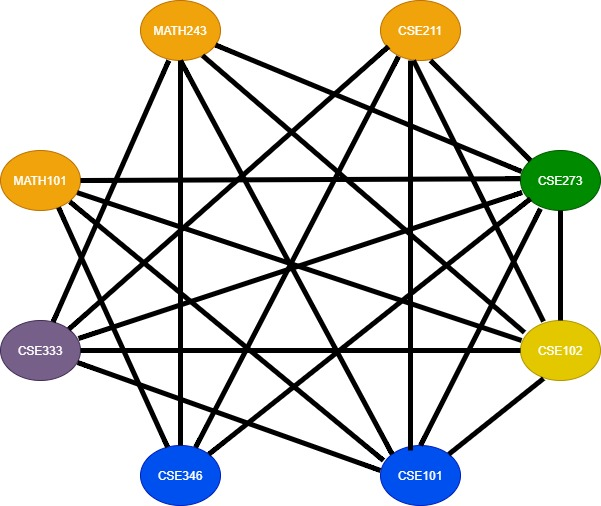
\includegraphics[height=4in]{newdia.jpg}
		\label{fig:G1a}
	\end{subfigure}%
\end{figure*}
\begin{itemize}
	\item CSE 273 is linked to all other classes, in return CSE 273 needs to be given a unique color. We give CSE 273 its GREEN color.
	\item Since CSE101 is not linked to all classes except CSE346, we give these two lessons blue.
	\item CSE 102 is linked to all classes except CSE 346, so CSE 102 has a unique yellow color.
	\item Each pair of Math 101, Math 243 and CSE 211 are all unconnected and thus we can give the same color Orange to these classes.
	\item Finally one class CSE 333 is remaining that is connected to class of all previous colors, thus we need to assign a fifth color Purple to CSE 333.
	
	
\end{itemize}
\newline
\newline We require at least 5 colors to color the vertices of the graph and thus we require 5 different time slots, where each color represents a time slot.
\newline
\newline
\newline Time slot 1: MATH101, MATH 243 and CSE 211
\newline Time slot 2: CSE 333
\newline Time slot 3: CSE 273
\newline Time slot 4: CSE 346 and CSE 101
\newline Time slot 5: CSE 102

\newpage
\problem{4: Applications for Hasse Diagram of Relations}{40}
Remember the Problem 3 in Homework 2. 
\newline
\newline
Write an algorithm to draw Hasse diagram of the given relations in "input.txt" which is given for HW2.
\newline
\newline
Your code should meet the following requirements, standards and accomplish the given tasks.


\begin{itemize}
	\item Read the relations from the text file "input.txt". You can use your code from HW2 if you implemented to read the file. If you didn't implement it, please check HW2 to learn how to read the relations from the file. 
	\item Determine each relation in "input.txt" whether it is reflexive, symmetric, anti-symmetric and transitive with your algorithm from HW2.
	\item In order to draw Hasse diagram, each relation must be POSET. Hence, the relation obeys the following rules:
	
	\begin{itemize}
		\item Reflexivity
		\item Anti-symmetric
		\item Transitivity 
	\end{itemize}
	If the relation is not a POSET, your algorithm is responsible to CONVERT it to POSET. 
	\begin{itemize}
		\item If the relation is not reflexive, add new pairs to make the relation reflexive.
		\item If the relation is symmetric, remove some pairs which make the relation symmetric. For instance, if the relation has (a, b) and (b, a), remove one of them randomly.
		\item If the relation is not transitive, add new pairs which would make the relation transitive. 
	\end{itemize}
	\item After the relation becomes POSET, your algorithm should obtain Hasse diagram of the relation and write the diagram with the following format. 
	\begin{itemize}
		\item An example of the output format is given in "exampleoutput.txt". The file has the result of the first relation in "input.txt".
		\item In "output.txt", each new Hasse diagram starts with "n".
		\item The relation is (a, a), (a, b), (a, e), (b, b), (b, e), (c, c), (c, d), (d, d), (e, e)
		\item The relation is already a POSET so we don't need to add or remove any pairs.
		\item After "n", write the POSET in the next line as it is shown in "exampleoutput.txt".
		\item Since the relation is POSET, it becomes (a, b), (b, e), (c, d) after removing reflexive and transitive pairs. 
		\item The following lines give each pair of Hasse diagram.
	\end{itemize}	
	\item You can implement your algorithm in Python, Java, C or C++.
	\item $\textbf{Important: }$ Put comments almost for each line of your code to describe what the line is going to do. 
	\item You should put your source code file (file name is problem1.$\{.c, .java, .py, .cpp\}$) and output.txt into your homework zip file (check Course Policy).
\end{itemize}



\end{document} 
